\documentclass[letter]{article}

\usepackage{fullpage}
\usepackage{url}

\title{Performance investigation}

\usepackage[pdftex]{graphicx}
\usepackage{multirow}
\usepackage{caption}
\usepackage{subcaption}

\begin{document}
\maketitle

\section{Disjoint set}

%Test Id = 3 512 pairs communication of 64 source nodes [0-63] to 512 destination nodes [512-1023]. Each source node sends data to 4 destination nodes e.g rank 0 sends data to ranks 512, 513, 514, 515. 1 rank per node, message size = 8MB. Total data amount transferred is 4GB = 512 x 8 MB. Chunk size for OPTIQ is 64 KB.

\section{Subset tests}

Subset Test Id = 87. Among N nodes, N/2 source nodes send data to N/16 destination nodes. The destination nodes are among the source nodes. There are N/2 pairs of communication, 8 MB of data per pair. There is 1 MPI/PAMI rank per node. Experiments are done for N=512, 1024, 2048, 4096 and 8192 nodes.

\begin{figure}[!htb]
\vspace{-0.1in}
\centering
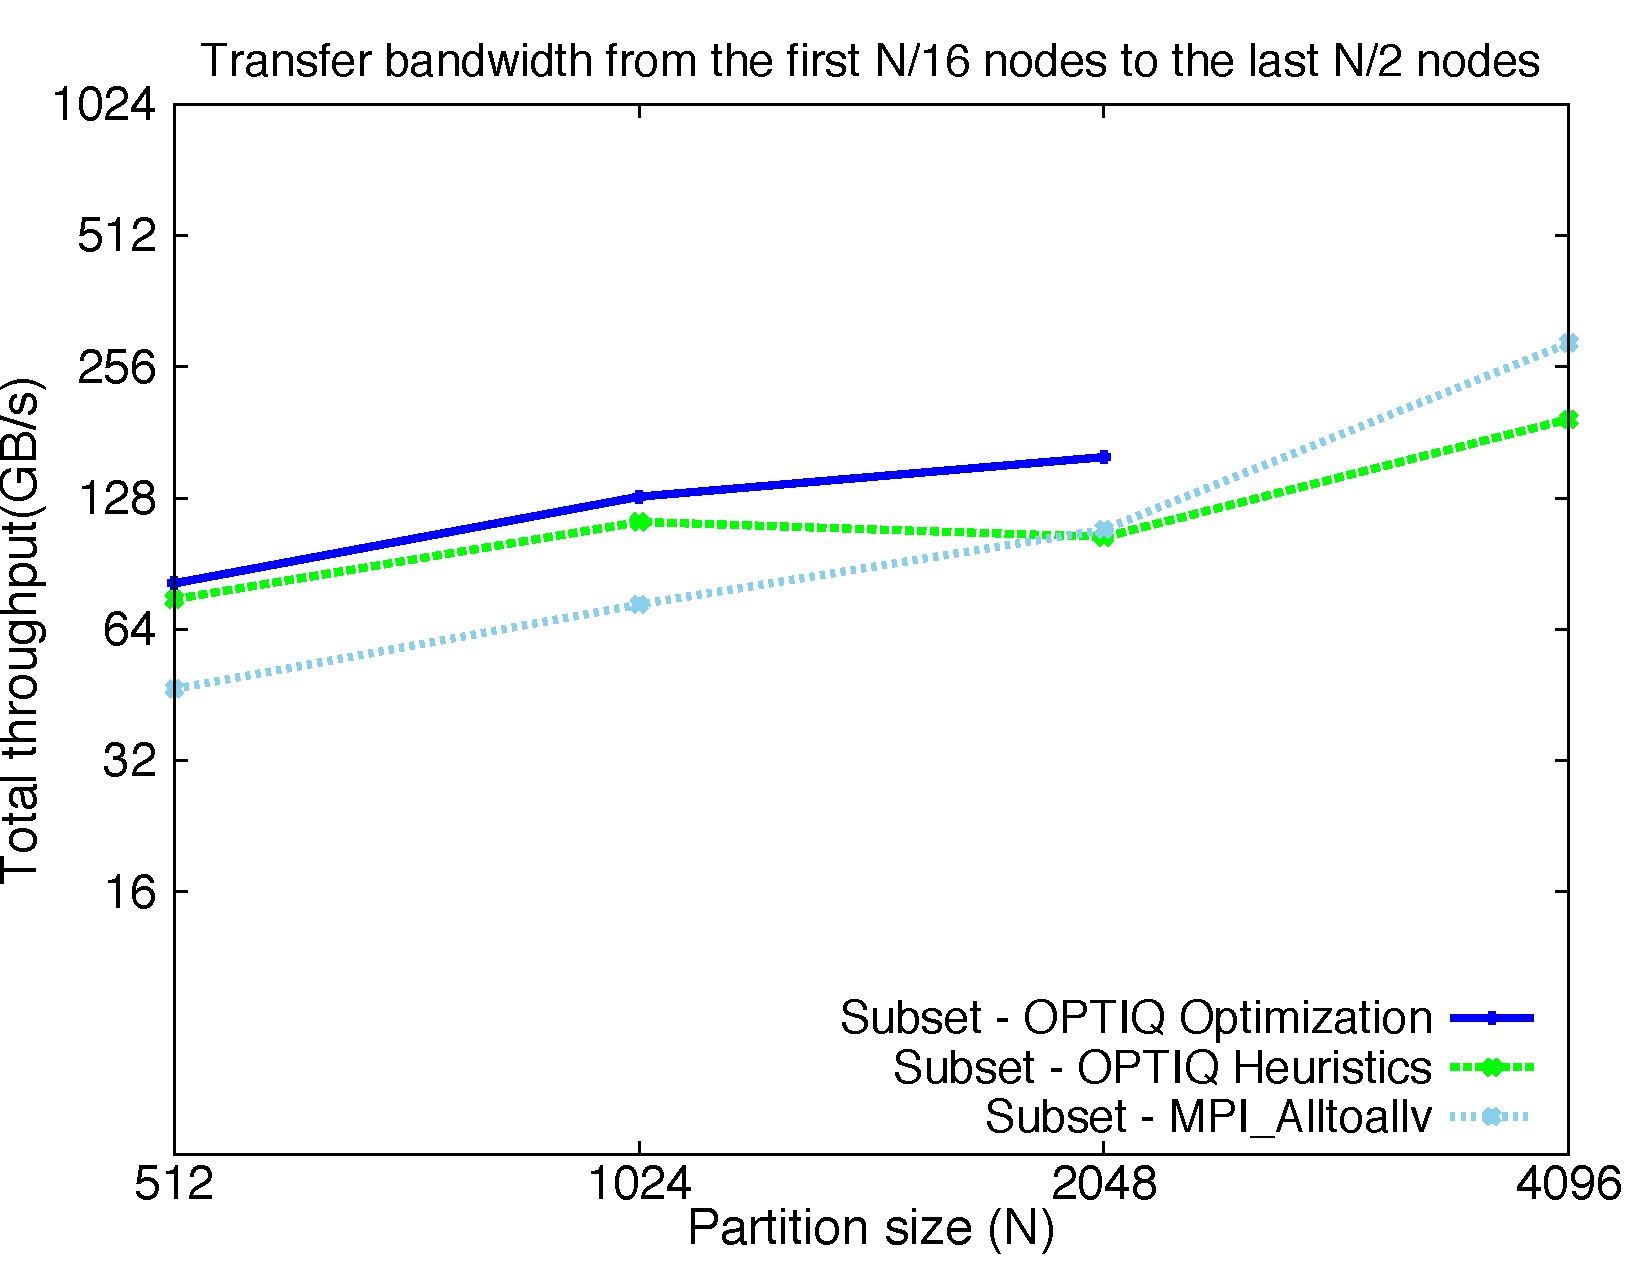
\includegraphics[scale=0.30]{report_figures/constantr_subset.pdf}
\vspace{-0.1in}
\caption{Subset performance}
\vspace{-0.1in}
\label{fig:patterns}
\end{figure}

\subsection {Total number of nodes 512}

Source nodes are the first 256 nodes (nodes 0 to 255), destination nodes are 32 nodes in the middle of the source nodes (nodes 128 to 159). There are 256 pairs of communication, 8 MB of data per pair. As 32 destination nodes are contiguous, per each node out of 10 links, 6 links along C, D, E dimensions are used for internal interconnection (connect nodes among 32 nodes). The 4 remaining links along A and B dimensions are used to interconnect with nodes outside of the destination set. Thus, the maximum achievable throughput is 32 (nodes) x 4 (links/node) x 1.7 (GB/s/link) = 217.6 (GB/s). The experiments were carried with Optimization, Heuristics and MPI\_Alltoallv. Table \ref{table:512_perf} shows the performance and path-related information. Table \ref{table:512_hopcopy} and \ref{table:512_load} show number of hops, number of copies and loads of the experiments. Figure \ref{fig:512_histo} shows the histogram (distribution) of number of hops, number of copies, number of paths sharing physical links and total amount of data traveling through a physical link.

Table \ref{table:512_perf} shows that Optimization throughput (83 GB/s) is a slightly higher than Heuristics (71 GB/s), and both are significantly higher than MPI\_Alltoallv (47 GB/s). It also shows that Optimization used 621 paths, Heuristics used 397 paths and MPI used 256 paths. Per job, Optimization has highest max, median and average number of paths. Because Optmization has highest number of paths, it also has highest total number of hops. However per path, the max, min, average and median number of of hops are very similar among Optimization, Heuristics and MPI\_Alltoallv, shown in Table \ref{table:512_hopcopy} and Figure \ref{fig:512_hop}. 

When data travels along the paths, it is split into small chunks, copied and injected again to the interconnect network at intermediate nodes. The number of copies can cause some delays thus, degrade throughput. In comparison to Heuristics, Optimization has higher total of number of copies but lower max, min, average and median number of copies per node, shown in Table \ref{table:512_load} and Figure \ref{fig:512_copy}. This is because it used more paths and nodes and thus spreaded the copies over more nodes. This can lead to better performance for Optmization.

Regarding loads over physical links, we consider two types of load on physical links: the number of paths that use a physical link and the actual amount of data travels through a physical link, shown in Table \ref{table:512_load}. While the number of paths load only reveals how many paths use a particular link, it does not reveal how much data actual travels through that particular link, which is more important in investigating performance. As the Table \ref{table:512_load} and Figure \ref{fig:512_loadpath} \& \ref{fig:512_loaddata}  show, Optmization has highest number paths per physical link, but it actually has lowest actual amount of data load. This is because Optimization split the data among paths and thus led to more balanced data load.

\begin{table}[h]
    \centering
    \begin{tabular}{ | l | p{0.75cm} | p{1.0cm} | p{1.0cm} | p{0.75cm} | p{0.5cm} | p{0.5cm} | p{0.5cm} | p{0.5cm} |}
    \hline
    \multirow{3}{*}{Type} & \multicolumn{3}{ c| }{Performance} & \multicolumn{5}{ c| }{Num. of Paths} \\ \cline{2-9}
    & Data (MB) & Time ($\mu$s) & BW (MB/s)& \multirow{2}{1cm}{Total Paths} & \multicolumn{4}{ c| }{Per Job} \\ \cline{6-9}
    & & & & & Max & Min & Avg & Med \\ \hline
    OPT & 2048 & 24524 & 83510    & 621 & 5 & 1 & 2.42 & 2 \\ \hline
    HEU & 2048 & 28765 & 71197    & 397 & 4 & 1 & 1.55 & 1 \\ \hline
    MPI & 2048 & 42837 & 47808    & 256 & 1 & 1 & 1.00 & 1 \\ \hline
    \end{tabular}
    \caption{Performance with number of paths in 512 nodes experiments}
    \label{table:512_perf}
\end{table}

\begin{table}[h]
    \centering
    \begin{tabular}{ | l | p{0.75cm} | p{0.5cm} | p{0.5cm} | p{0.5cm} | p{0.5cm} | p{1.0cm} | p{0.75cm} | p{0.5cm} | p{1.0cm} | p{0.5cm} |}
    \hline
    \multirow{3}{*}{Type} & \multicolumn{5}{ c| }{Num. of Hops} & \multicolumn{5}{ c| }{Num. of Copies} \\ \cline{2-11}
    & \multirow{2}{1cm}{Total hops} & \multicolumn{4}{ c| }{Per Path} & \multirow{2}{1cm}{Total copies} & \multicolumn{4}{ c| }{Per Node} \\ \cline{3-6} \cline{8-11}
    & & Max & Min & Avg & Med & & Max & Min & Avg & Med \\ \hline
    OPT &  3099 & 8 & 1 & 4.99 & 5 & 128862 & 1218 & 4  & 397.80 & 301\\ \hline
    HEU &  1863 & 8 & 1 & 4.69 & 5 & 123478 & 1472 & 32 & 400.90 & 320\\ \hline
    MPI &  1024 & 8 & 1 & 4.00 & 4 &	    &      &    &        &    \\ \hline
    \end{tabular}
    \caption{Number of hops and copies in 512 nodes experiments}
    \label{table:512_hopcopy}
\end{table}

\begin{table}[h]
    \centering
    \begin{tabular}{ | l | p{0.75cm} | p{0.5cm} | p{0.5cm} | p{0.75cm} | p{0.5cm} | p{1.5cm} | p{1.25cm} | p{1.25cm} |  p{1.25cm} |}
    \hline
     &  \multicolumn{5}{ c| }{Load (Num of Paths)} & \multicolumn{4}{ c| }{Actual Load (Data Amount) per Link} \\ \hline
    Type & Total & Max & Min & Avg & Med & Max & Min & Avg & Med \\ \hline
    OPT & 1201 & 9 & 1 & 2.58 & 2 & 15597568 & 65536 & 8376830 & 7929856 \\ \hline
    HEU & 1030 & 3 & 1 & 1.81 & 2 & 25165824 & 2097152 & 9224144 & 8388608 \\ \hline
    MPI & 384 & 6 & 1 & 2.67 & 2 & 16777216 & 8388608 & 8388608 & 8388608 \\ \hline
    \end{tabular}
    \caption{Load: number of paths and actual total amount of data over physical links in 512 nodes experiments}
    \label{table:512_load}
\end{table}

\begin{figure}[h]
        \centering
        \begin{subfigure}[b]{0.49\textwidth}
                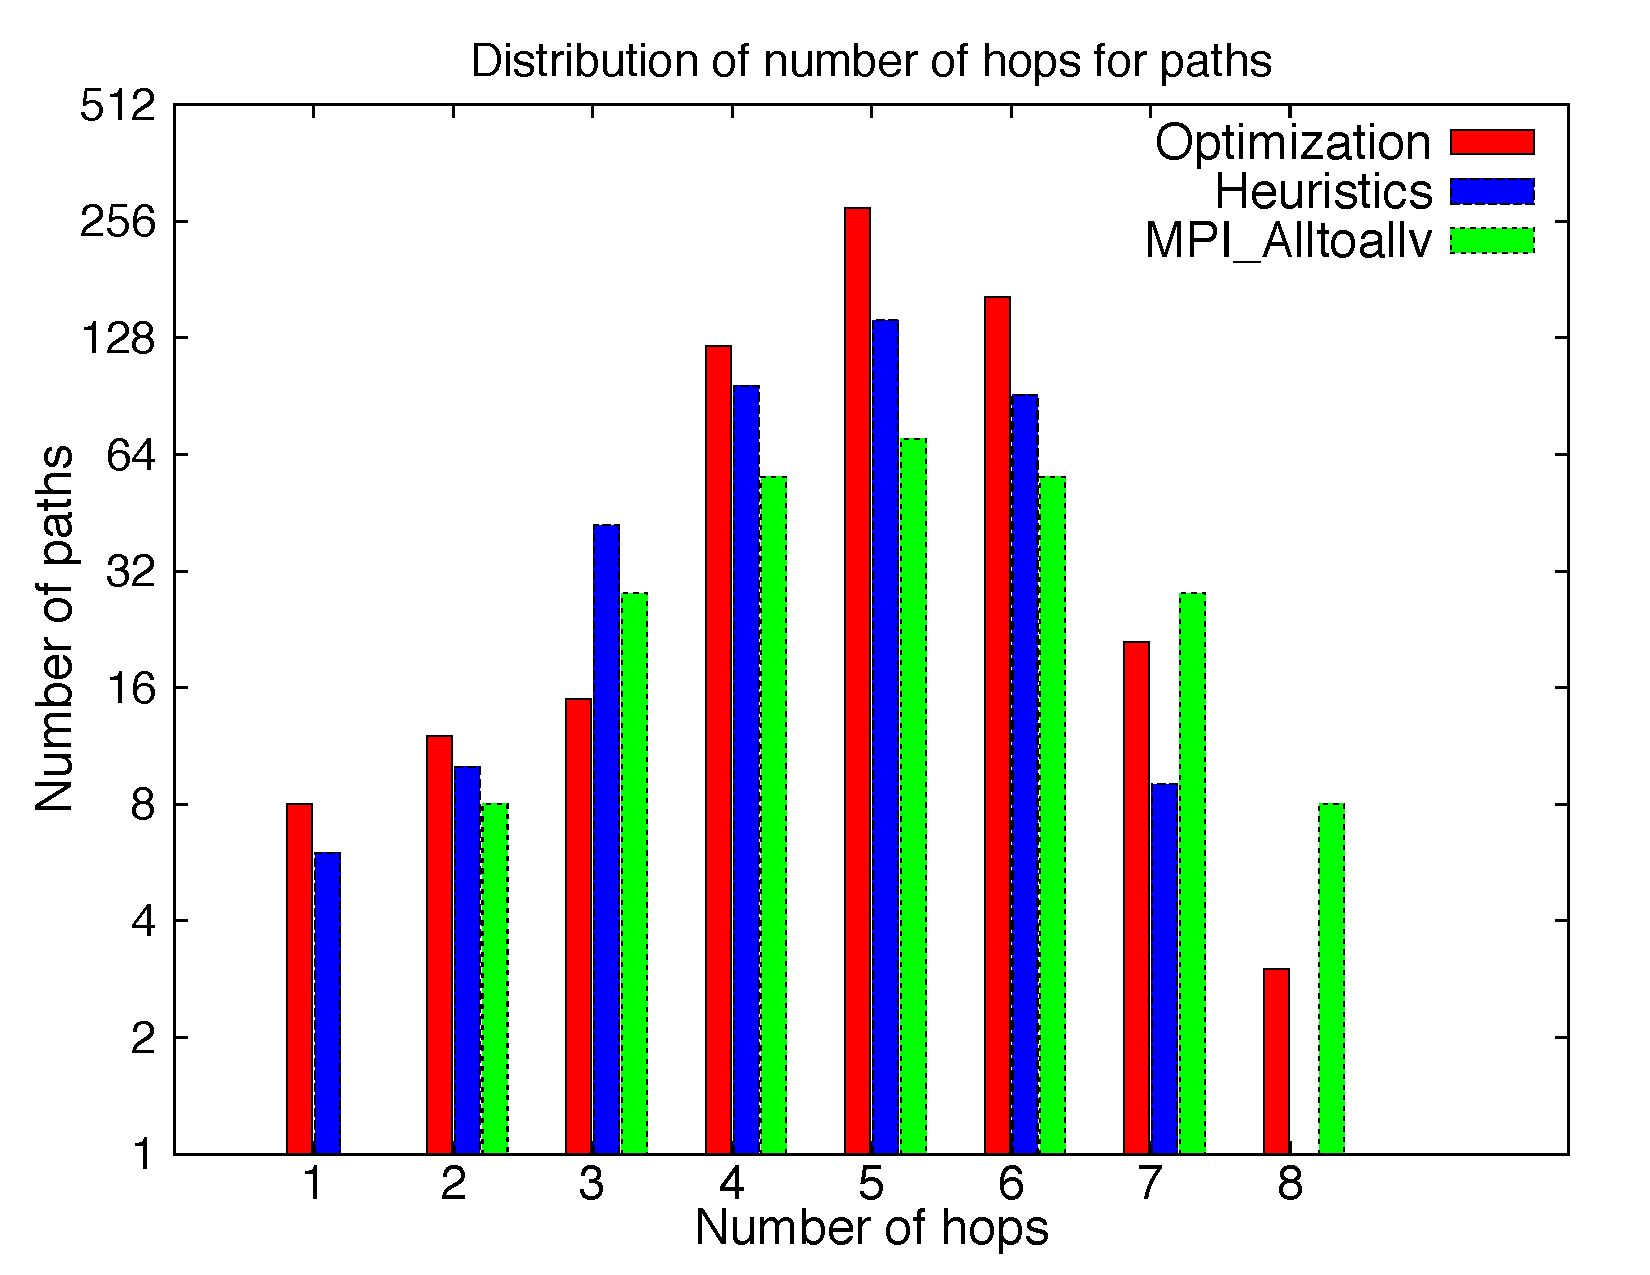
\includegraphics[width=\textwidth]{report_figures/hop_histo.pdf}
                \caption{Distribution of number of hops over paths}
                \label{fig:512_hop}
        \end{subfigure}%
        ~ %add desired spacing between images, e. g. ~, \quad, \qquad, \hfill etc.
          %(or a blank line to force the subfigure onto a new line)
        \begin{subfigure}[b]{0.49\textwidth}
                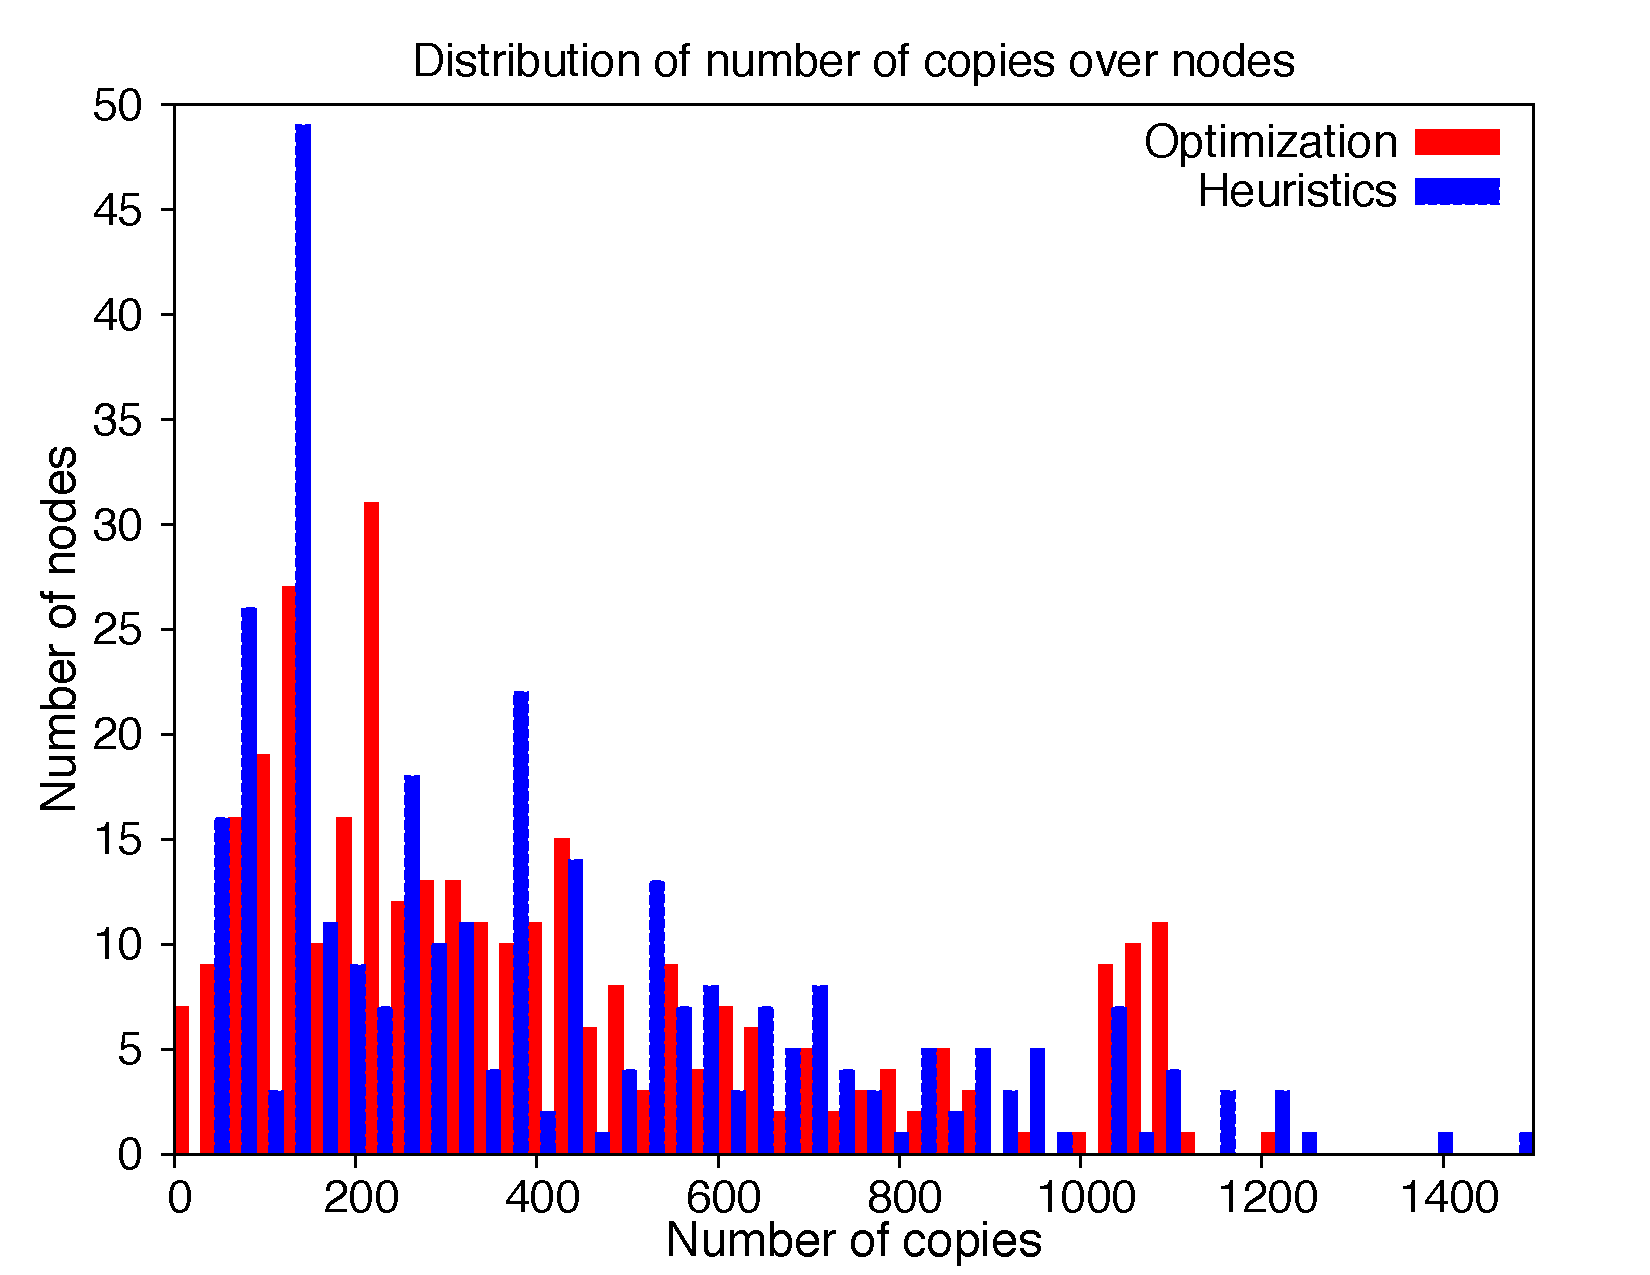
\includegraphics[width=\textwidth]{report_figures/copy_histo.pdf}
                \caption{Distribution of number of copies over nodes}
                \label{fig:512_copy}
        \end{subfigure}
        ~ %add desired spacing between images, e. g. ~, \quad, \qquad, \hfill etc.
          %(or a blank line to force the subfigure onto a new line)
        \begin{subfigure}[b]{0.49\textwidth}
                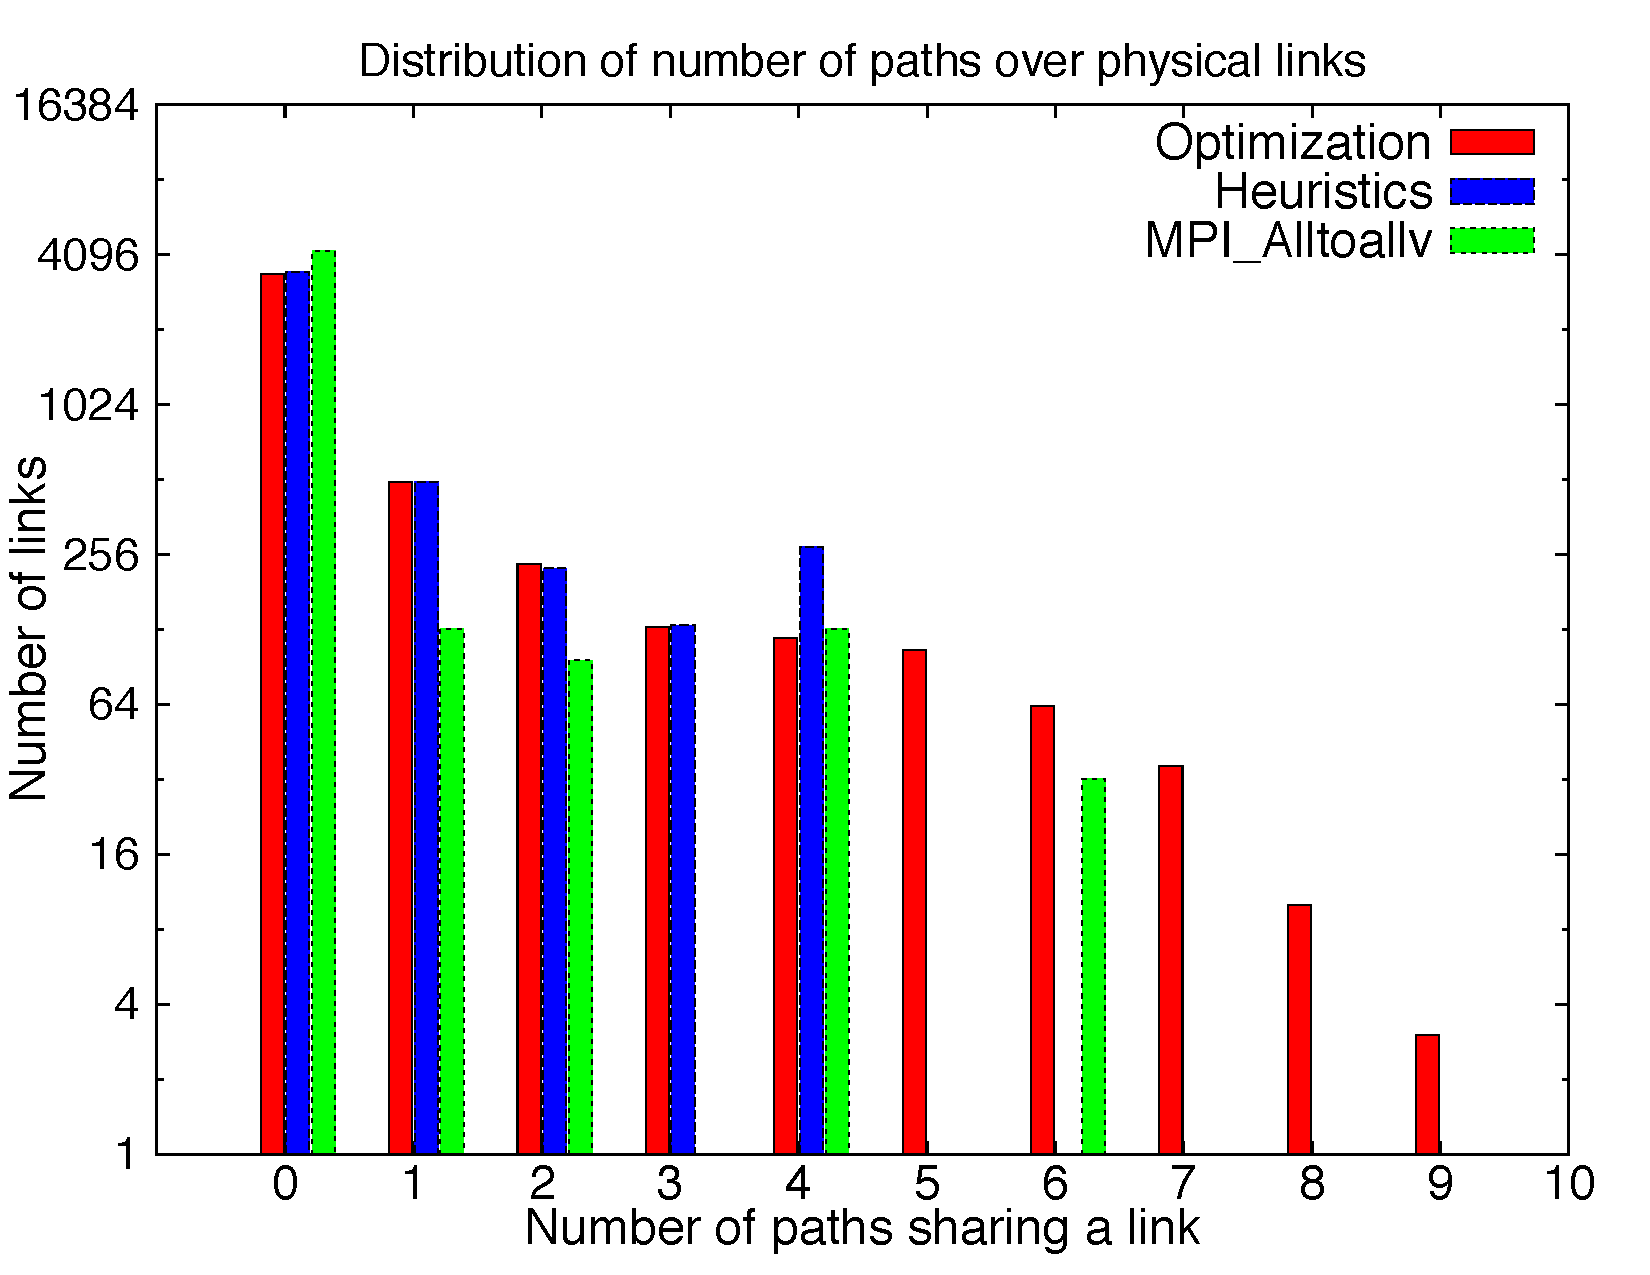
\includegraphics[width=\textwidth]{report_figures/loadpath_histo.pdf}
                \caption{Distribution of number of paths over physicallinks}
                \label{fig:512_loadpath}
        \end{subfigure}
	~ %add desired spacing between images, e. g. ~, \quad, \qquad, \hfill etc.
          %(or a blank line to force the subfigure onto a new line)
	\begin{subfigure}[b]{0.49\textwidth}
                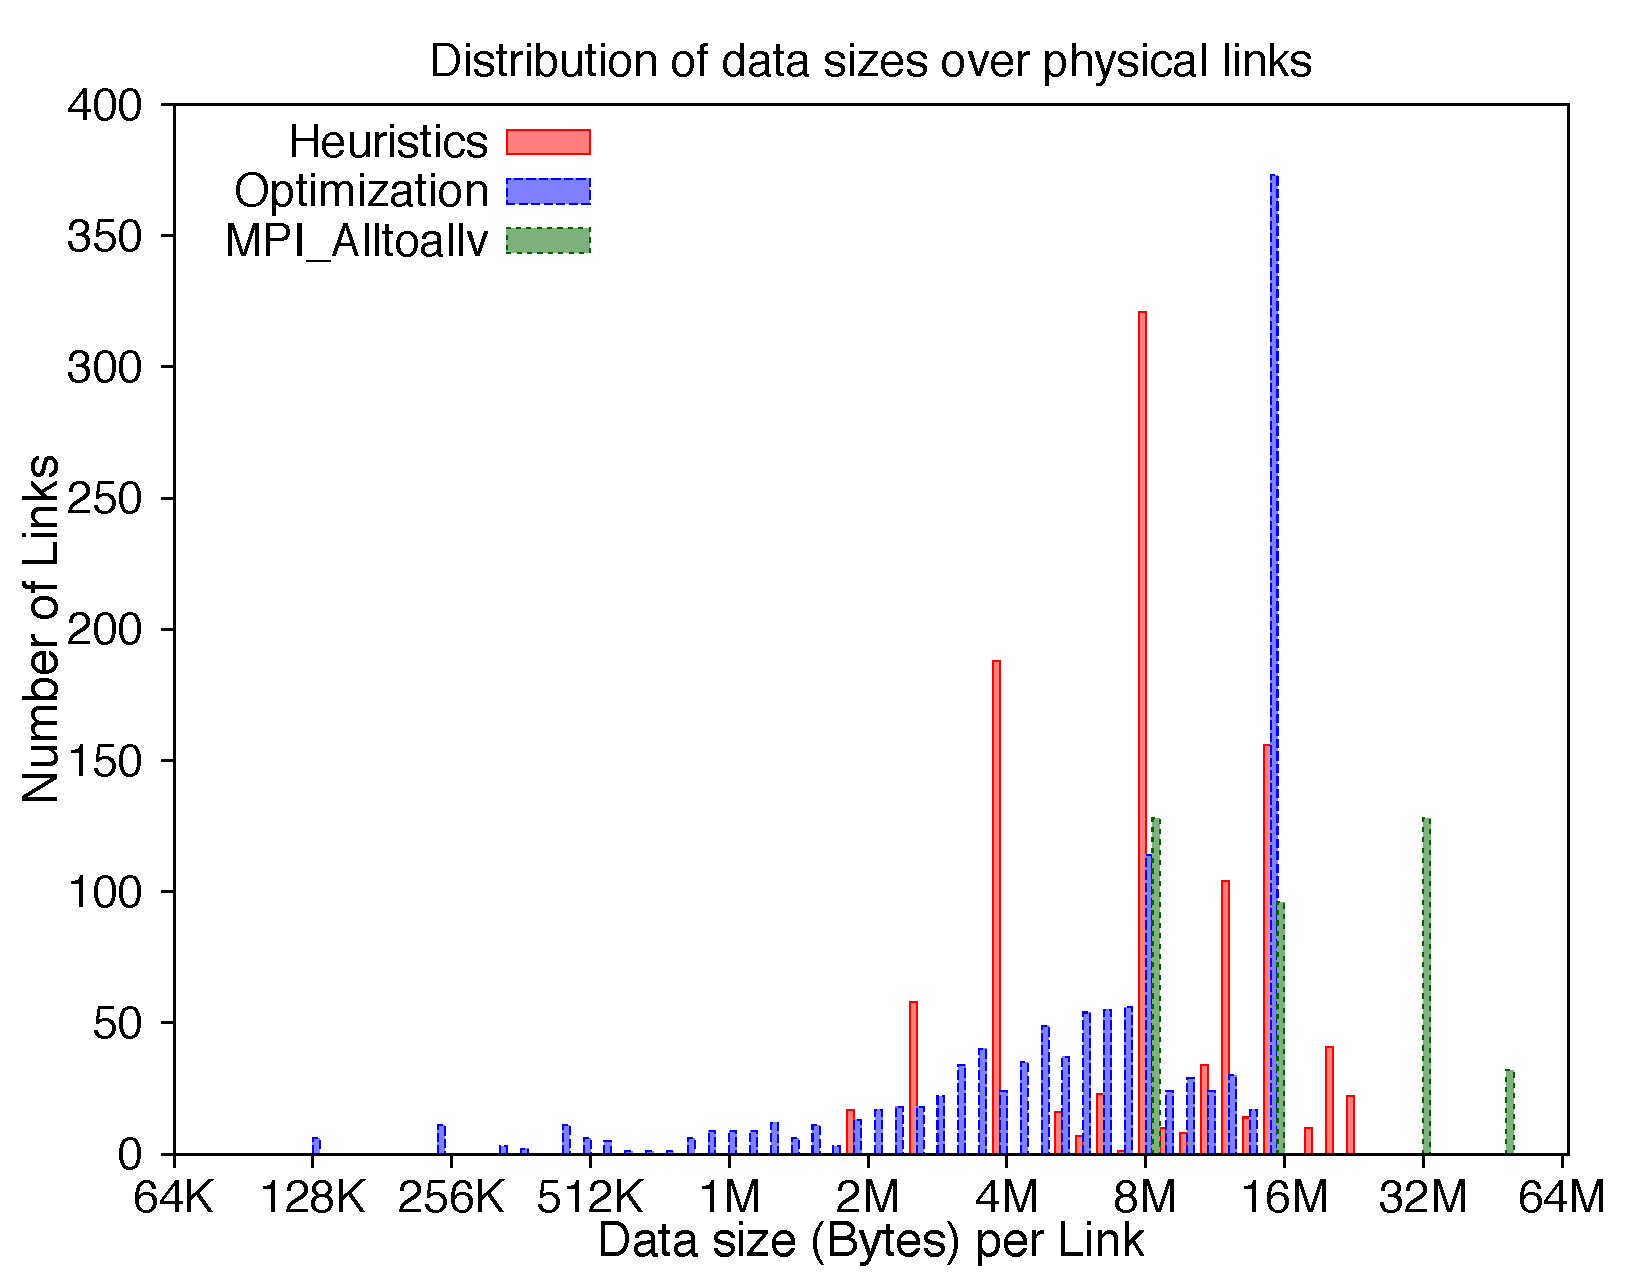
\includegraphics[width=\textwidth]{report_figures/loaddata_histo.pdf}
                \caption{Distribution of total data size over physical links}
                \label{fig:512_loaddata}
        \end{subfigure}
        \caption{Historgram of hops, copies, load in terms of number of paths and data size}\label{fig:animals}
	\label{fig:512_histo}
\end{figure}

In conclusion, Optimization throughput (83 GB/s) is a slightly higher than Heuristics (71 GB/s), and both are significantly higher than MPI\_Alltoallv (47 GB/s). The reasons include:
\begin{itemize}
\item Optimization and Heuristics used more paths than MPI\_Alltoallv. MPI\_Alltoallv has only 256 paths, Heuristics has 397 and Optimization has 621 - Table \ref{table:512_perf}.
\item Optimization and Heursitcs has lower maximum load than MPI\_Alltoallv in terms of total amount of data over physical links. The maximum number of paths sharing in case of Optimization is 9 which is higher than both Heuristics (at most 3 paths per link) and MPI\_Alltoallv (at most 6 paths per link). However, because we split data on different paths in case of Optimization, we ended up with least maximum total amount of data per link. That contributes to better performance for Optimization - Table \ref{table:512_load} and Figure \ref{fig:512_loadpath} \& \ref{fig:512_loaddata}.
\item They all have approximately number of hops (max, min, avg and med) - Table \ref{table:512_hopcopy} and Figure \ref{fig:512_hop}.
\item Optimization has lower maximum number of copies and the copies ditribution is better than Heuristics - Table \ref{table:512_hopcopy} and Figure \ref{fig:512_copy}.
\end{itemize}

\subsection {Paritition size 2048}

128 sources node sends data to 1024 destination nodes. 8 MB of data for each pair of communication.

\begin{center}
    \begin{tabular}{ | l | p{0.75cm} | p{1cm} | p{0.75cm} | p{0.75cm} | p{0.5cm} | p{0.5cm} | p{0.5cm} | p{0.5cm} | p{0.75cm} | p{0.9cm} | p{0.5cm} | p{0.5cm} | p{0.5cm} | p{0.5cm} |}
    \hline
     &  \multicolumn{2}{ c| }{Performance} &  & \multicolumn{5}{ c| }{Num. of Hops} & \multicolumn{6}{ c| }{Load} \\ \hline
    Type & Time (us) & BW (MB/s) & Num. Paths & Total hops & Max & Min & Avg & Med & Total load & Loaded links & Max & Min & Avg & Med \\ \hline
    MPI & 73731 & 111105 & 1024 & 7168 & 14 & 1 & 7.00 & 7 & 7168 & 1448 & 16 & 1 & 4.95 & 5 \\ \hline
    HEU & 76790 & 106680 & 2603 & 18070 & 14 & 1 & 6.94 & 6 & 18070 & 5133 & 7 & 1 & 3.52 & 3 \\ \hline
    OPT & 50339 & 162736 & 2441 & 18843 & 14 & 1 & 7.72 & 8 & 18843 & 5056 & 16 & 1 & 3.73 & 3 \\
    \hline
    \end{tabular}
\end{center}

\end{document}
